\documentclass{article}
\usepackage{amsmath}
\usepackage{amssymb}
\usepackage[a4paper, top=25mm, bottom=25mm, left=25mm, right=25mm]{geometry}
\usepackage{pgfplots}
\pgfplotsset{compat=1.18}
\usepackage{mathtools}
\usepgfplotslibrary{polar}
\usepgfplotslibrary{fillbetween}

\begin{document}
\large

\begin{center}
2021-2022 Spring \\MAT124 Final\\(23/05/2022)
\end{center}

\noindent 1. Find the largest and smallest values of $f(x,y) = x^2+y^2$ subject to the constraint $x+y=1$ with $x\geq0$ and $y\geq0$.

\hfill

\noindent 2. Sketch the region corresponding to the double integral

\begin{equation*}
    \int_0^{\frac{1+\sqrt5}{2}}\int_{\sqrt{y}}^{\sqrt{1-y^2}}\,dx\,dy
\end{equation*}

\hfill

\noindent and reverse the order of integration. Do not evaluate the integral!

\hfill

\noindent 3. Sketch the region inside the circle $r=1$ and outside the cardioid $r=1+\sin\theta$ and then, using a double integral, find the area of the region.

\hfill

\noindent 4. Using a double integral, find the volume of the solid bounded above by the sphere $x^2+y^2+z^2 = 16$ and below by the circular region $x^2+y^2\leq2$ in the $xy$-plane.

\hfill

\noindent 5. Let us consider the frustum of the cone $z=\sqrt{x^2+y^2}$ between the planes $z=1$ and $z=2$.

\hfill

\noindent (i) Sketch the graph of the frustum.

\hfill

\noindent (ii) Find the surface area of the frustum.

\hfill

\noindent 6. Let $S$ be the region in the cylinder $x^2+y^2 = 1$ bounded above by the plane $z=6$ and below by the paraboloid $z=1-x^2-y^2$.

\hfill

\noindent (i) Using the spherical coordinates, set up (but do not evaluate!) an integral for the volume of the solid $S$.

\hfill

\noindent (ii) Using the cylindrical coordinates, find the volume of the solid $S$.

\newpage

\begin{center}
Solutions (Last update: 7/22/25 (22nd of July) 11:15 PM)
\end{center}

\noindent 1) Let $g(x,y)=x+y-1$ and then, solve the system of equations below using the method of Lagrange multipliers.

\[
\left.
\begin{array}{ll}
\displaystyle\nabla f =\lambda \nabla g \\
\displaystyle g(x,y) = 0
\end{array}
\right\}\quad
\begin{array}{ll}
\nabla f = \left\langle 2x, 2y\right\rangle = \lambda\left\langle1,1\right\rangle = \lambda\nabla g\\\therefore\displaystyle \lambda = 2x\quad \text{and}\quad \lambda = 2y\quad \text{and}\quad x+y-1=0
\end{array}
\]

\[\lambda=2x=2y\implies x=y\]
\[x+y-1=0 \,\rightarrow\, 2x-1 = 0\,\rightarrow\,x=\frac12=y\]

\hfill

\noindent Evaluate $\displaystyle f\left(\frac12,\frac12\right)$ to find the minimum value.

\[f\left(\frac12,\frac12\right)=\left(\frac12\right)^2+\left(\frac12\right)^2=\frac12\]

\hfill

\noindent $f(x,y)$ is defined for $x\geq0$ and $y\geq0$. This implies that $0\leq y \leq1$ and $0\leq x\leq1$ by the constraint. The domain of $f$ is closed and bounded, and $f$ is continuous. By the extreme value theorem, the absolute minima and maxima must exist. Using the method of Lagrange multipliers, we could find only one point. This means that the other value exists on the boundary of $f$.

\[x=0\,\rightarrow\,0+y-1=0\,\rightarrow\,y=1,\quad y=0\,\rightarrow\, x+0-1=0\,\rightarrow\, x=1\]
\[f(0,1) = 0^2 +1^2 = 1,\quad f(1,0) = 1^2+0^2 = 1\]

\hfill

\noindent Eventually, compare the values we obtain.

\[\boxed{\frac12\,\text{is the absolute minimum}, 1\,\text{is the absolute maximum}.}\]

\hfill

\noindent 2)

\begin{center}
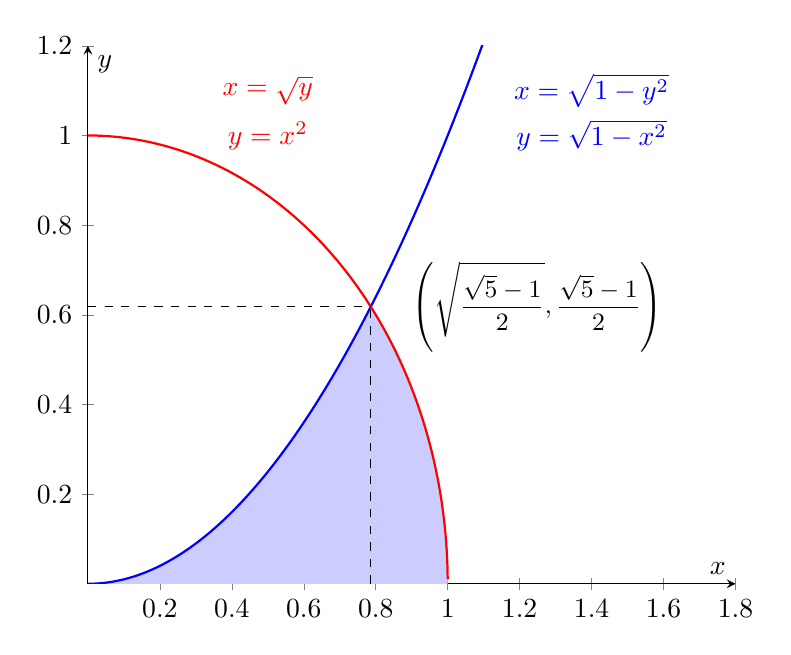
\begin{tikzpicture}
  \begin{axis}[
      axis lines=center,
      xlabel={$x$},
      ylabel={$y$},
      xmin=0, xmax=1.8,
      ymin=0, ymax=1.2,
      samples=200,
      clip=true,
      scale=1.2,
    ]
    
    \addplot [
        fill=blue!20,
        domain=0:0.786,
        draw=none,
    ] {x^2} \closedcycle;
    
    \addplot [
        fill=blue!20,
        domain=0.784:1,
        draw=none,
    ] {sqrt(1-x^2)} \closedcycle;

    \addplot [
        thick,
        blue,
        domain=0:1.1,
        samples=200,
    ] {x^2};

    \addplot [
        thick,
        red,
        domain=0:1.1,
        samples=3200,
    ] {sqrt(1-x^2)};

    \node[blue] at (axis cs:1.4,1.1) {$x = \sqrt{1 - y^2}$};
    \node[red] at (axis cs:0.5,1.1) {$x = \sqrt{y}$};
    \node[blue] at (axis cs:1.4,1) {$y = \sqrt{1 - x^2}$};
    \node[red] at (axis cs:0.5,1) {$y=x^2$};
    \node at (axis cs:1.25,0.618) {\small$\displaystyle\left(\sqrt{\frac{\sqrt5-1}{2}},\frac{\sqrt5-1}2\right)$};

    % Label y-max
    \draw[dashed] (axis cs:0,0.618) -- (axis cs:{sqrt(0.618)},0.618);
    \draw[dashed] (axis cs:0.786,0) -- (axis cs:0.786,0.618);

    \node[left] at (axis cs:0,0.618) {\footnotesize $\frac{-1+\sqrt{5}}{2}$};

  \end{axis}
\end{tikzpicture}
\end{center}

\hfill

\noindent The integral with reverse order is as follows.

\begin{equation*}
\boxed{\int_0^{\sqrt{\frac{\sqrt5 - 1}2}}\int_0^{x^2}\,dy\,dx + \int_{\sqrt{\frac{\sqrt5 - 1}2}}^{1}\int_0^{\sqrt{1-x^2}}\,dy\,dx}
\end{equation*}

\hfill

\noindent 3) Find where these two curves intersect and then find the area.

\[1=1+\sin\theta\implies\sin\theta=0\implies\theta=k\pi,\quad k\in\mathbb{Z}\]


\begin{center}
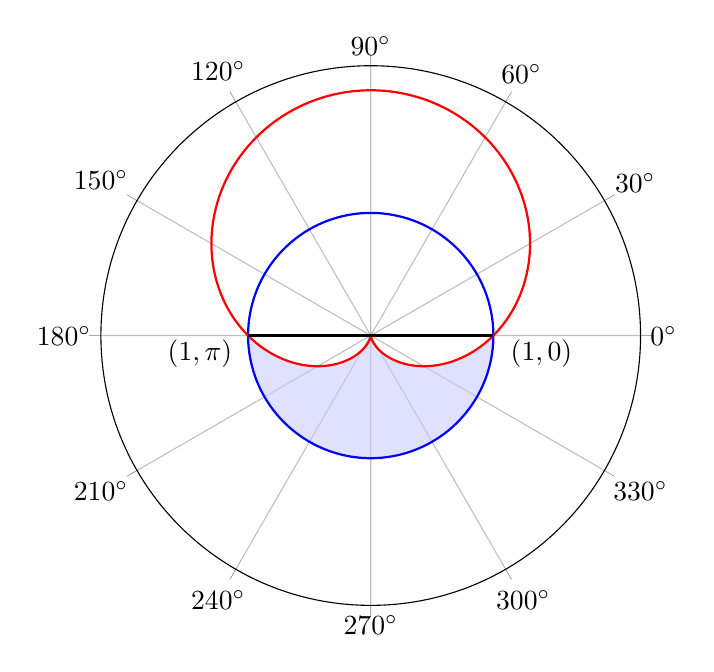
\begin{tikzpicture}
  \begin{polaraxis}[ytick=\empty, axis y line=none, xticklabel=$\pgfmathprintnumber{\tick}^\circ$,]
    \addplot [
      domain=pi:2*pi,
      samples=300,
      draw=none,
      name path=A,
      data cs=polarrad,
    ] {1};

    \addplot [
      domain=pi:2*pi,
      samples=300,
      draw=none,
      name path=B,
      data cs=polarrad,
    ] {1+sin(deg(x))};

    \addplot [
      blue!20,
      fill opacity=0.6,
    ] fill between[of=A and B];

    \addplot [
      domain=0:2*pi,
      samples=300,
      thick,
      blue,
      data cs=polarrad,
    ] {1};

    \addplot [
      domain=0:2*pi,
      samples=300,
      thick,
      red,
      data cs=polarrad,
    ] {1+sin(deg(x))};

    \draw[black, thick] (axis cs: 0,-1) -- (axis cs: 0,1);
    \node at (axis cs: 6,-1.4) {$(1,\pi)$};
    \node at (axis cs: -6,1.4) {$(1,0)$};

  \end{polaraxis}
\end{tikzpicture}
\end{center}

\begin{align*}
\text{Area}&=\frac12\int_\pi^{2\pi}\left[1^2-(1+\sin\theta)^2\right]\,d\theta=\frac12\int_\pi^{2\pi}\left[-2\sin\theta-\sin^2\theta\right]\,d\theta\,\,\left[\sin^2x+\cos^2x=1\right]\\\\&=-\int_\pi^{2\pi}\sin\theta\,d\theta-\frac12\int_\pi^{2\pi}(1-\cos^2\theta)\,d\theta\quad[2\cos^2\theta-1=\cos(2\theta)] \\\\&=-\int_\pi^{2\pi}\sin\theta\,d\theta+\int_\pi^{2\pi}\frac{\cos(2\theta)-1}{4}\,d\theta=\int_\pi^{2\pi}\left[-\frac14+\frac14\cos(2\theta)-\sin\theta\right]\,d\theta\\\\&=\left[-\frac\theta4+\frac18\sin(2\theta)+\cos\theta\right]_{\pi}^{2\pi}=\left[\left(-\frac{\pi}2+0+1\right)-\left(-\frac{\pi}4+0-1\right)\right]={\boxed{2-\frac{\pi}4}}
\end{align*}

\hfill

\noindent 4) We have the sphere $x^2+y^2+z^2=16$. So, the upper bound is $z=\sqrt{16-x^2-y^2}$, while the lower bound is $z=0$. If we project the domain onto the $xy$-plane, we see that the upper and lower bounds for $y$ are $\sqrt{2-x^2}$ and $-\sqrt{2-x^2}$, respectively. For $x$, the integration starts from $-\sqrt2$ and ends at $\sqrt2$. The volume of the object can be evaluated using the following integral.

\hfill

\begin{equation*}\mathrm{I}=\int_{-\sqrt2}^{\sqrt2}\int_{-\sqrt{2-x^2}}^{\sqrt{2-x^2}}\left[\sqrt{16-x^2-y^2}-0 \right]\,dy\,dx\end{equation*}

\hfill

\noindent This integral seems a little bit hard. We can switch to polar coordinates for ease. Use the transformation below.

\[
\begin{array}{c}
x^2+y^2=r^2\\
dA=dy\,dx =r\,dr\,d\theta
\end{array}\quad\rightarrow\quad
\begin{array}{c}
0\leq z\leq\sqrt{16-r^2}\\
0\leq r\leq \sqrt2\\
0\leq\theta\leq 2\pi\\
\end{array} 
\]

\begin{align*}\mathrm{I}&=\int_{0}^{2\pi}\int_{0}^{\sqrt{2}}\sqrt{16-r^2}\,r\,dr\,d\theta=\int_{0}^{2\pi}\left[-\frac13\left(16-r^2\right)^{3/2}\right]_{r=0}^{r=\sqrt2}\,d\theta\\\\&=\frac13\int_0^{2\pi}\left[-14^{3/2}-\left(-16^{3/2}\right)\right]\,d\theta=\boxed{\frac{2\pi}{3}\left(16^{3/2}-14^{3/2}\right)}
\end{align*}

\hfill

\noindent 5)

\hfill

\noindent (i)
\begin{center}
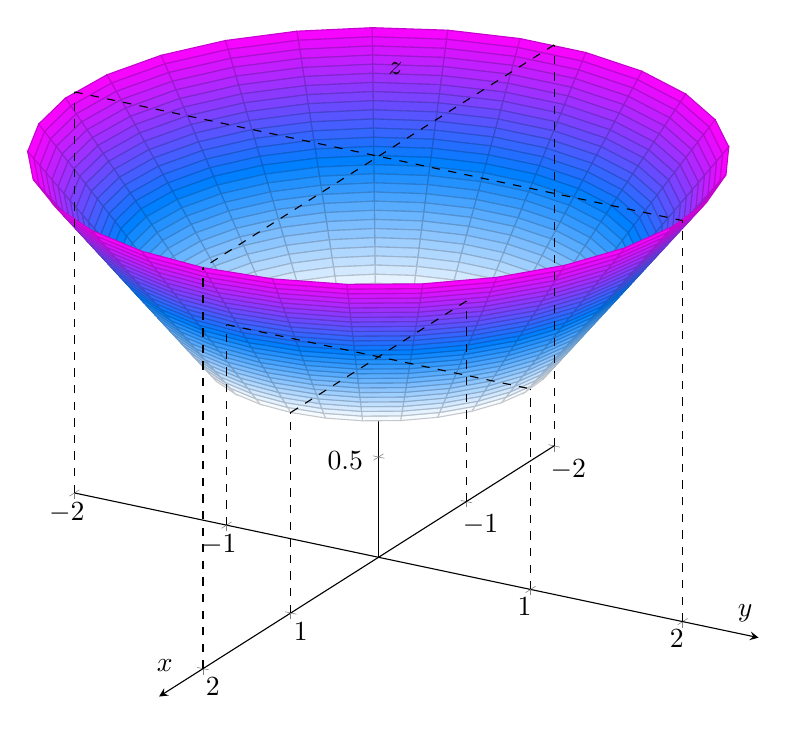
\begin{tikzpicture}
  \begin{axis}[
    view={120}{30},
    axis lines=center,
    xlabel={$x$},
    ylabel={$y$},
    zlabel={$z$},
    xtick={-2,-1,1,2},
    ytick={-2,-1,1,2},
    xmin=-2, xmax=2.5,
    ymin=-2, ymax=2.5,
    zmin=0, zmax=2.5,
    samples=30,
    domain=0:360,
    colormap/cool,
    scale=2,
  ]
    \addplot3[
      surf,
      z buffer=sort,
      y domain=1:2,
    ]
    ({y*cos(x)}, {y*sin(x)}, {y});
%\addplot3[y domain=0:1, dashed, samples = 10]({y*cos(x)}, {y*sin(x)}, {y});
    
\draw[dashed] (axis cs:0,-2,2) -- (axis cs: 0, 2, 2);
\draw[dashed] (axis cs:-2,0,2) -- (axis cs: 2, 0,2);
\draw[dashed] (axis cs:-1,0,1) -- (axis cs: 1, 0, 1);
\draw[dashed] (axis cs:0,-1,1) -- (axis cs: 0, 1,1);

\draw[dashed] (axis cs:-2,0,0) -- (axis cs: -2, 0, 2);
\draw[dashed] (axis cs:0,2,0) -- (axis cs: 0,2,2);
\draw[dashed] (axis cs:2,0,0) -- (axis cs: 2, 0, 2);
\draw[dashed] (axis cs:0,-2,0) -- (axis cs: 0, -2,2);

\draw[dashed] (axis cs:-1,0,0) -- (axis cs: -1, 0, 1);
\draw[dashed] (axis cs:0,1,0) -- (axis cs: 0,1,1);
\draw[dashed] (axis cs:1,0,0) -- (axis cs: 1, 0, 1);
\draw[dashed] (axis cs:0,-1,0) -- (axis cs: 0, -1,1);

\end{axis}
\end{tikzpicture}
\end{center}

\hfill

\noindent (ii) Using the double integral below, we find the lateral surface area.

\begin{align*}
A&=\iint_D\sqrt{1+\left(\frac{\partial z}{\partial x}\right)^2 +\left(\frac{\partial z}{\partial y}\right)^2}\,dA= \iint_D\sqrt{1+\left(\frac{x}{\sqrt{x^2+y^2}}\right)^2 +\left(\frac{y}{\sqrt{x^2+y^2}}\right)^2}\,dA \\\\&=\iint_D\sqrt{1+\left(\frac{x^2+y^2}{x^2+y^2}\right)}\,dA=\iint_D\sqrt{1+1}\,dA=\sqrt{2}\iint_D\,dA
\end{align*}

\hfill

\noindent If we switch to polar coordinates, we can easily evaluate the integral.

\begin{equation*}A=\sqrt2\int_0^{2\pi}\int_1^2\,r\,dr\,d\theta=\sqrt2\int_0^{2\pi}\left[\frac{r^2}2\right]_{r=1}^{r=2}\,d\theta=\sqrt2\int_0^{2\pi}\frac32\,d\theta=3\pi\sqrt2\end{equation*}

\hfill

\noindent The radii of the top and bottom surface are $r=2$ and $r=1$, respectively. The total surface area is $3\pi\sqrt2 + \pi\left(2^2+1^2\right)=\boxed{3\pi\sqrt2+5\pi}$

\hfill

\noindent 6)

\hfill

\noindent (i) For spherical coordinates, we have

\[
\begin{array}{c}
z=\rho\cos\theta\\
r=\rho\sin\theta\\
x^2+y^2+z^2=\rho^2\\
dV=\rho^2\sin\phi\,d\rho\,d\phi\,d\theta
\end{array}\quad\rightarrow\quad
\begin{array}{c}
x^2+y^2=1\,\rightarrow\,\rho^2\sin^2\phi = 1\\
z=6\,\rightarrow\,\rho\cos\phi=6\\
z=1-x^2-y^2\,\rightarrow\,\rho\cos\phi=1-\rho^2\sin^2\phi
\end{array}
\]

\hfill

\noindent We have the lower bound for $\rho$, which is the solution of $\rho\cos\phi=1-\rho^2\sin^2\phi$

\[
\begin{array}{c}
\rho\cos\phi=1-\rho^2\sin^2\phi\\\\
\rho^2\sin^2\phi+\rho\cos\phi-1=0\\\\
\displaystyle \rho_{1,2} = \frac{-\cos\phi \pm\sqrt{\cos^2\phi-4\cdot\sin^2\phi\cdot(-1)}}{2\sin^2\phi}\quad\left[x_{1,2}=\frac{-b\pm\sqrt{b^2-4ac}}{2a}\right]\\\\
\displaystyle \rho>0\implies\rho_{\text{lower}}=\frac{-\cos\phi +\sqrt{\cos^2\phi+4\sin^2\phi}}{2\sin^2\phi}
\end{array}
\]

\hfill

\noindent However, we have two distinct upper bounds for $\phi$. We need to find the value of $\phi$ where the surfaces $\rho\cos\phi = 6$ and $\rho^2\sin^2\phi=1$ intersect.

\begin{equation*}
\rho^2\sin^2\phi=1 \,\rightarrow\,\rho\sin\phi = 1
\end{equation*}

\[
\left.
\begin{array}{c}
\rho\sin\phi=1\\
\rho\cos\phi=6
\end{array}
\right\}\quad\tan\phi=\frac16\implies\phi=\arctan{\frac16}
\]

\hfill

\noindent For $\displaystyle\phi<\arctan\frac16$, the upper bound is $\displaystyle \frac6{\cos\theta}$. Meanwhile, for $\displaystyle\phi>\arctan\frac16$, it is $\displaystyle \frac1{\sin\theta}$.

\hfill

\noindent The region in the $xy-$plane is circular, therefore $0\leq\theta\leq2\pi$. As for $\phi$, we have $\displaystyle0\leq\phi\leq\frac{\pi}2$. The volume of the object in spherical coordinates can be expressed as follows.

\begin{equation*}
\boxed{\begin{array}{cc}
V=&\displaystyle\int_0^{2\pi}\int_0^{\arctan{\textstyle\frac16}}\int_{\textstyle\frac{-\cos\phi +\sqrt{\cos^2\phi+4\sin^2\phi}}{2\sin^2\phi}}^{\textstyle\frac6{\cos\phi}}\,\rho^2\sin\phi\,d\rho\,d\phi\,d\theta\\
&\displaystyle+\int_0^{2\pi}\int_{\arctan{\textstyle\frac16}}^{\pi/2}\int_{\textstyle\frac{-\cos\phi +\sqrt{\cos^2\phi+4\sin^2\phi}}{2\sin^2\phi}}^{\textstyle\frac1{\sin\phi}}\,\rho^2\sin\phi\,d\rho\,d\phi\,d\theta 
\end{array}}
\end{equation*}

\hfill

\noindent In fact, we are looking for the minimum value of the upper bound for $\phi$ between $\displaystyle\frac1{\sin\theta}$ and $\displaystyle\frac6{\cos\theta}$. Hence, we can write the equivalent expression as follows.

\begin{equation*}
\boxed{V=\displaystyle\int_0^{2\pi}\int_0^{\pi/2}\int_{\textstyle\frac{-\cos\phi +\sqrt{\cos^2\phi+4\sin^2\phi}}{2\sin^2\phi}}^{\min\left(\textstyle\frac6{\cos\phi},\frac1{\sin\phi}\right)}\,\rho^2\sin\phi\,d\rho\,d\phi\,d\theta}
\end{equation*}

\hfill

\noindent (ii) For cylindrical coordinates, we have

\[
\begin{array}{c}
z=z\\
r^2=x^2+y^2\\
dV=r\,dz\,dr\,d\theta
\end{array}\quad\rightarrow\quad
\begin{array}{c}
x^2+y^2=1\,\rightarrow\,r^2 = 1\,\rightarrow\,r=1\\
z=6\\
z=1-x^2-y^2\,\rightarrow\,z=1-r^2
\end{array}
\]

\hfill

\noindent The volume can be expressed as follows.

\begin{align*}
    V&=\int_0^{2\pi}\int_0^1\int_{1-r^2}^{6}\,r\,dz\,dr\,d\theta=\int_0^{2\pi}\int_0^1\big[z\big]_{z=1-r^2}^{z=6}\,r\,dr\,d\theta\\\\&=\int_0^{2\pi}\int_0^1\left(r^3+5r\right)\,dr\,d\theta=\int_0^{2\pi}\left[\frac{r^4}{4} + \frac{5r^2}{2}\right]_{r=0}^{r=1}\,d\theta\\\\&=\big[\theta\big]_0^{2\pi}\cdot\left[ \left(\frac{1^4}4 + \frac{5\cdot1^2}2\right)-\left(0\right)\right]=\boxed{\frac{11\pi}2}
\end{align*}

\end{document}